%
%     hw5_bbordwell.tex
%     Baylee Bordwell (baylee.bordwell@colorado.edu)
%     Based on the template by Benjamin Brown (bpbrown@colorado.edu)
%     Aug 27, 2014
%
%     Problem set 5 for ASTR/ATOC 5540, Mathematical Methods, taught at
%     University of Colorado, Boulder, Fall 2014.
%
%

\documentclass[10pt, preprint]{aastex}
% formatting based on 2014 NASA ATP proposal with Jeff Oishi

%%%%%%begin preamble
\usepackage[hmargin=1in, vmargin=1in]{geometry} % Margins
\usepackage{hyperref}
\usepackage{url}
\usepackage{times}
\usepackage{natbib}
\usepackage{graphicx}
\usepackage{amsmath}
\usepackage{amsfonts}
\usepackage{amssymb}
\usepackage{pdfpages}
\usepackage{import}
% for code import
\usepackage{listings}
\usepackage{color}
\usepackage{ragged2e}

\hypersetup{
     colorlinks   = true,
     citecolor     = gray,
     urlcolor       = blue
}

%% headers
\usepackage{fancyhdr}
\pagestyle{fancy}
\lhead{ASTR/ATOC 5540}
\chead{}
\rhead{name: Baylee Bordwell}
\lfoot{Problem Set 5}
\cfoot{\thepage}
\rfoot{Fall 2014}
% no hline under header
\renewcommand{\headrulewidth}{0pt}

\newcommand{\sol}{\ensuremath{\odot}}

% make lists compact
\usepackage{enumitem}
%\setlist{nosep}

%%%%%%end preamble


\begin{document}
\section*{Problem Set 5: Detrending Kepler Data, part II}
\begin{enumerate}
\item Done!

\item The fits begin to significantly diverge for polynomials of degree 4 or 5. As shown in the figure, the QR method becomes significantly better around polynomials of degree 6.
\begin{figure}[!ht]
  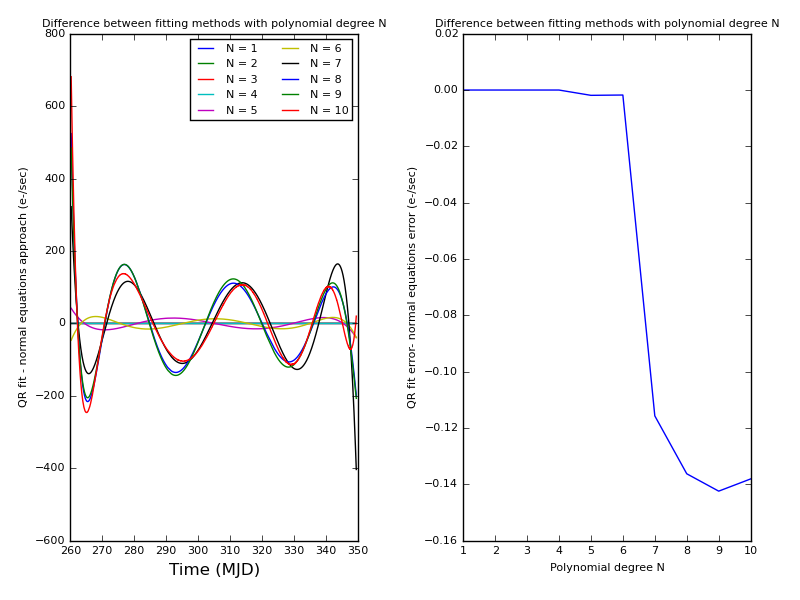
\includegraphics[width=4in]{hw5_fig1.png}
\end{figure}

\item The times are different...but not too different.
\begin{figure}[!ht]
  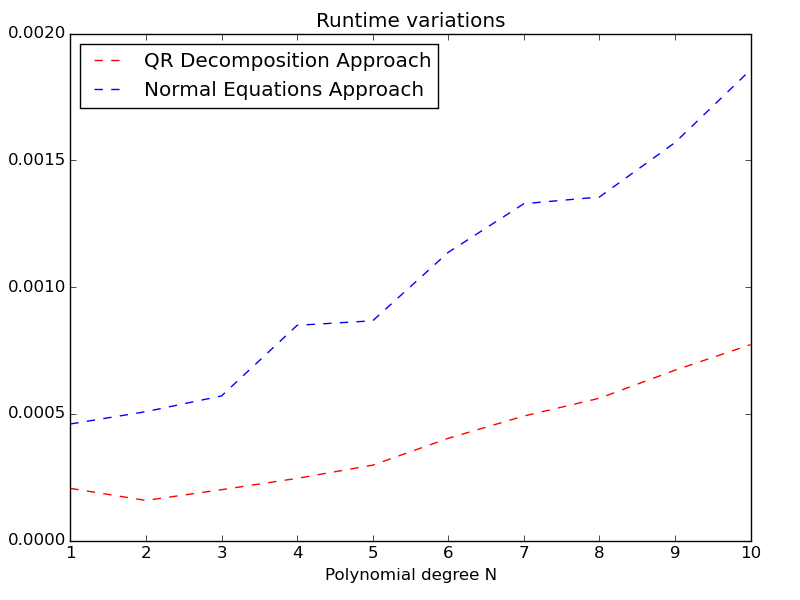
\includegraphics[width=4in]{hw5_fig2.png}
\end{figure}

\item Written (although the conjugate gradient doesn't work...yet.). Even shifting the polynomial by a linear offset, say the average of the data, is inordinately helpful as a first guess, and does not rely on previous solutions.

\item SOR is working, and finds a solution of [2.52977039e+05  -2.29478198e+02   2.88131707e-01]
with $\omega$ = 1.9 at a tolerance of $1e-4$ in 41505 steps and 7 seconds for a preconditioned matrix. This compares with the QR and normal equations solutions,
 QR: [  2.52984806e+05  -2.29529965e+02   2.88217303e-01]
 NE: [  2.52984806e+05  -2.29529965e+02   2.88217303e-01]
And now that I've realized I'm a total spacecase (I matched the keyword for Gauss-Seidel to the Jacobi method), Gauss-Seidel is also working, and finds a solution of at a tolerance of 1e-4 in 637581 steps and 3167 seconds for a preconditioned matrix (my computer is intolerably slow).

\item I changed x0 for the SOR method (as if you look at the time required for Gauss-Seidel on my laptop, I think you'll understand why I refuse to test this out...), and didn't find a significant difference. Sadly, my program also crashed on the plotting step...and I really don't want to rerun it, so I still only have the convergence plot for SOR.

And as there was only one fit, there is not much to comment on, other than the fact that I would expect more movement over- and undershooting 0, so I worry for the veracity of this plot.
\begin{figure}[!ht]
  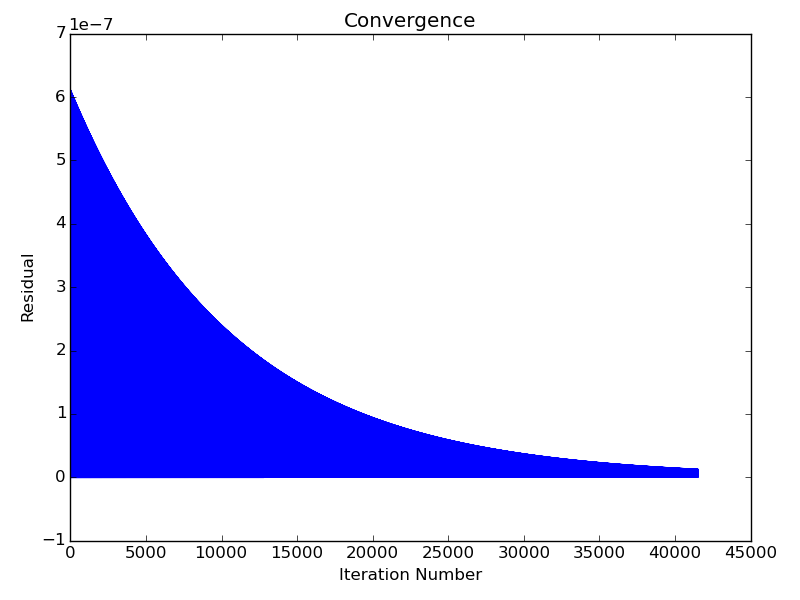
\includegraphics[width=4in]{hw5_fig3.png}
\end{figure}

\end{enumerate}
\end{document}
